\chapter{需求建模 }
\section{数据流图}
\subsection{顶层数据流图}

\begin{figure}[ht]
\centering
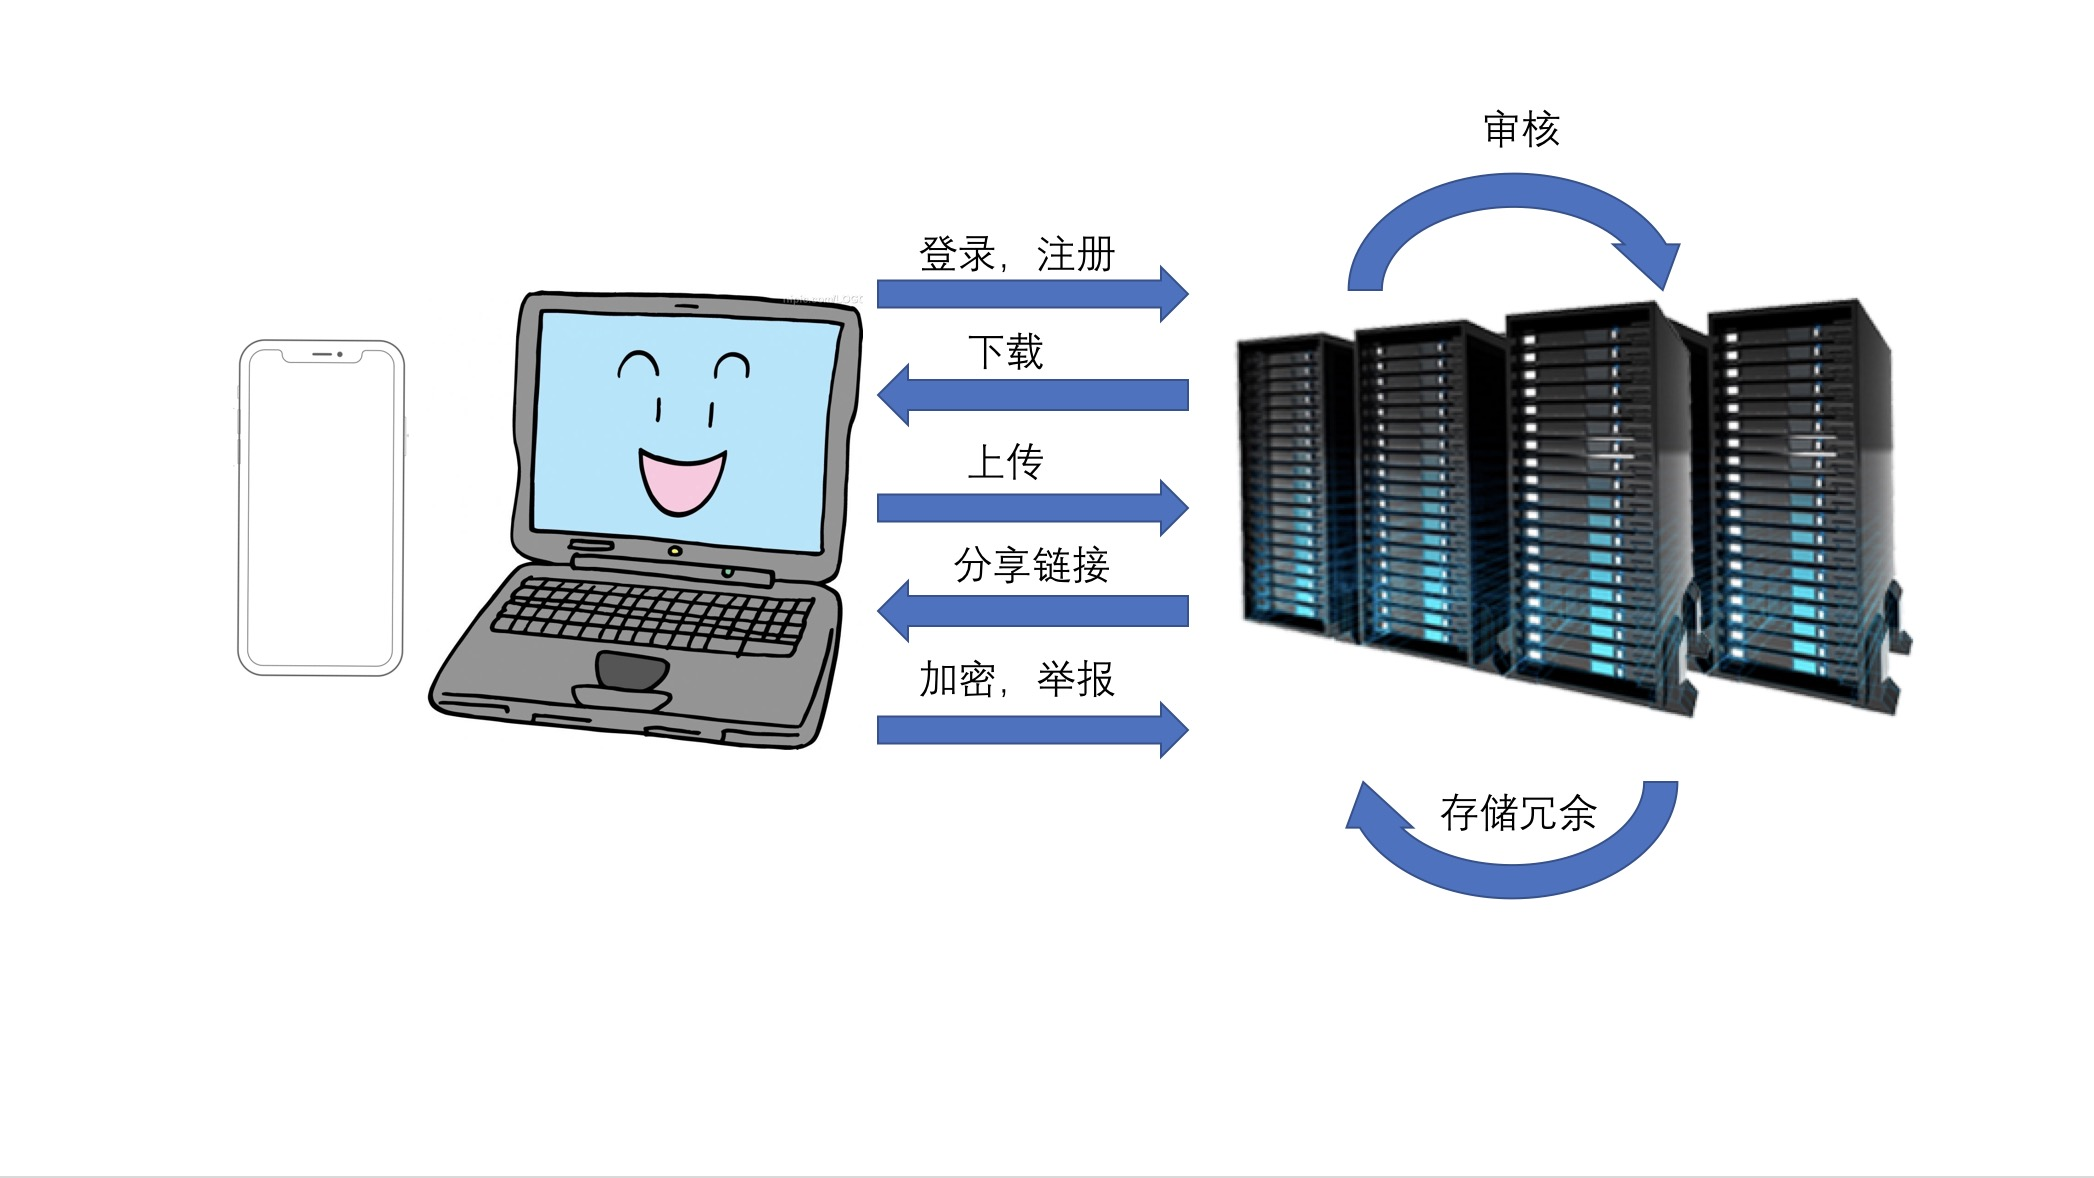
\includegraphics[width=16cm]{top.png}
\caption{顶层数据流图}\label{fig:noted-figure}
\end{figure}

\subsection{层数据流图}

在这里画出0层数据流图

\subsection{层数据流图}
<Draw the Level-1 DFD here>

在这里画出1层数据流图

\section{数据字典}
\subsection{数据流说明}
\subsubsection{数据流1名称}
<Title of  the data flow should accord with the one in data flow diagram, and the Data description notions should be used.  >

与数据流图中的名称一致,采用数据描述符号说明数据流的内容

\subsubsection{数据流2名称}
<Title of  the data flow should accord with the one in data flow diagram, and the Data description notions should be used   >

与数据流图中的名称一致,采用数据描述符号说明数据流的内容

\subsection{数据存储说明}
\subsubsection{数据存储1名称}
<Title of  the data flow should accord with the one in data flow diagram, and the Data description notions should be used. The arrangement of the data in data store should also be described.>

与数据流图中的名称一致,采用数据描述符号说明数据流的内容,另外还需描述数据排列方式

\subsubsection{数据存储2名称}
<Title of  the data flow should accord with the one in data flow diagram, and the Data description notions should be used.The arrangement of the data in data store should also be described.>

与数据流图中的名称一致,采用数据描述符号说明数据流的内容,另外还需描述数据排列方式

\subsection{加工说明}
\subsubsection{加工1名称}
<Use natural language, Decision table/Decision tree and Pseudocode to describe how to process the data flow>

采用自然语言,判断表/判断树,伪码的形式描述对数据流进行处理的过程

\subsubsection{加工2名称}
<Use natural language, Decision table/Decision tree and Pseudocode to describe how to process the data flow>

采用自然语言,判断表/判断树,伪码的形式描述对数据流进行处理的过程
